\documentclass[../TDAM3.tex]{subfiles}%

\begin{document}
\section{Galène}
\enonce{%
	L'élaboration du plomb par voie sèche repose sur l'extraction et l'exploitation
	d'un minerai appelé galène~: le sulfure plomb \ce{PbS}. Ce minerai cristallise
	selon une structure type \ce{NaCl}, avec \ce{S^{2-}} sur les nœuds d'un réseau
	CFC et \ce{Pb^{2+}} sur les sites octaédriques.
	\begin{tcn}(defi)<lftt>'l'{Données}
		$M_{\ce{Pb}} = \SI{207.2}{g.mol^{-1}}$~; $M_{\ce{S}} =
			\SI{32.1}{g.mol^{-1}}$~; densité $d = \num{7.62}$.
	\end{tcn}
}%
\QR{%
	Représenter la maille élémentaire de la galène.
}{%
	Voir figure.
	\begin{center}
		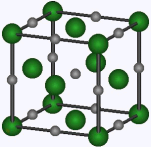
\includegraphics[scale=1]{galene}
		\captionof{figure}{Maille élémentaire de la galène. Les anions sont en vert,
			les cations en gris.}
		\label{fig:gal}
	\end{center}
}%

\QR{%
	Déterminer la coordinence de chacun des ions dans cette structure.
}{%
	En raisonnant sur un cation, par exemple au centre du cube, ses PPV sont
	sur les faces du cube (et forment l'octaèdre), distants de $a/2$~: les
	cations ont une coordinence de 6. \smallbreak
	En raisonnant sur un anion, par exemple au centre de la face avant, ses PPV
	sont les cations aux centres des arêtes (donc 4) \textbf{plus} les cations
	au centre des 2 mailles auquel cet anion appartient. Ainsi, les anions ont
	également une coordinence de 6.
}%

\QR{%
	Déterminer le paramètre de maille $a$ de la structure.
}{%
	La population d'une maille CFC est de $8\times1/8+6\times1/2=4$, donc on
	a 4 anions \ce{S^{2+}} en propre. On a également 4 sites O en propre
	$(1+12\times1/4)$, donc 4 cations \ce{Pb^{2+}}. Ainsi, la masse volumique
	vaut
	\[
		\rho = \frac{4M_{\ce{Pb}} + 4M_{\ce{S}}}{\Nc_A a^3}
		\qqdonc
		\boxed{a = \left( \frac{4(M_{\ce{Pb}} + M_{\ce{S}})}{\Nc_A\rho}
			\right)^{1/3} = \SI{596}{pm}}
	\]
}%

\end{document}
